\documentclass[../main.tex]{subfiles}
\begin{document}
\section*{Determine a Contrarre}

\textbf{Key Features of the Checklist }
\begin{enumerate}
    \item \textbf{Purpose and Scope}
    \begin{itemize}
        \item \textbf{Objective:} The checklist is used to assess the correctness and completeness of the "determina a contrarre" document. It ensures that the determination includes all necessary identifiers, normative references, and procedural details as mandated by legislation and municipal guidelines.
        \item \textbf{Possible Answers:} Reviewers must respond to each item with one of three possible answers: "SI" (Yes), "NO" (No), or "NON RICHIESTO" (Not Required), indicating whether the element is correctly included or applicable.
    \end{itemize}
    \item \textbf{Normative References}
    \begin{itemize}
        \item The checklist starts by listing a comprehensive set of legal references that must be considered when reviewing the document. These references include various legislative decrees, laws, and guidelines (e.g., D.Lgs. n. 267/2000, Legge n. 241/1990, D.L. 6 luglio 2012 n. 95, among others), as well as specific directives from regional and local bodies.
        \item These references provide the legal framework within which the determination must be evaluated, ensuring that all statutory and regulatory requirements are met.
    \end{itemize}
    \item \textbf{Evaluation Points Organized by Sections}
 The checklist is divided into several sections, each focusing on different aspects of the determination:
    \begin{itemize}
        \item \textbf{General Identifying Elements of the Act:}
        \begin{itemize}
            \item \textbf{Intestazione and Oggetto:} Verify that the document includes details about the issuing authority, the organizational structure (sector, service), and a clear subject line that includes the correct code and legal basis.
            \item \textbf{Identification Codes:} Ensure that unique identifiers like the CIG/CUP, CPV codes, and cost centers are correctly reported.
        \end{itemize}
        \item \textbf{Elements Related to the Issuing Entity:}
        \begin{itemize}
            \item \textbf{Authority and Delegation:} Check if the document includes details about the decree of appointment for the responsible manager or the delegation of signing authority if the signing is performed by someone other than the primary executive.
            \item \textbf{Designation of Responsible Personnel:} Confirm that the determination provides the required information for the nomination of the project manager (RUP) or any other responsible figure, along with contact details and relevant mandates.
        \end{itemize}
        \item \textbf{Normative References:}
        \begin{itemize}
            \item \textbf{Specific Norms:} Assess whether the determination explicitly cites the specific normative provisions (such as the Code of Public Contracts) that justify the content of the act.
            \item \textbf{General Norms and Principles:} Verify that general legal frameworks (e.g., TUEL, Legge n. 241/90) are included when necessary to support the logical structure of the determination.
            \item \textbf{Principles and Interpretative Norms:} Check the inclusion of guiding principles, especially those related to administrative discretion and the prioritization of results, as required by specific legislative articles.
        \end{itemize}
        \item \textbf{Typical Elements Specific to the Contracting Act:}
        \begin{itemize}
            \item \textbf{Procedural Details:} Evaluate if the document sets out clear deadlines for concluding the procedure and identifies the expected outcome of the contracting process.
            \item \textbf{Project Elements:} Check for detailed information on elements such as the object of the contract, execution costs, and the proposed economic framework, which include budget estimations and financial commitments.
            \item \textbf{Additional Technical and Environmental Criteria:} Ensure that any mandatory technical or environmental criteria (like DUVRI for safety, minimum environmental criteria for public contracts) are detailed.
        \end{itemize}
        \item \textbf{Accounting and Financial References:}
        \begin{itemize}
            \item \textbf{Budgetary and Financial Commitments:} Confirm that the determination includes references to the approved budget, any relevant financial authorizations (e.g., PEG, bilancio pluriennale), and ensures compliance with public finance rules.
            \item \textbf{Transparency in Financial Reporting:} Verify that details regarding expenditure, funding, and any ANAC contributions are explicitly stated.
        \end{itemize}
        \item \textbf{Transparency and Anti-Corruption Measures:}
        \begin{itemize}
            \item \textbf{Publication Requirements:} Check whether the determination meets transparency obligations, such as the publication of acts on the official online bulletin (Albo Pretorio Online).
            \item \textbf{Regularity Certifications:} Ensure that the document indicates that it will be forwarded for financial regularity checks, as required by law.
        \end{itemize}
        \item \textbf{Formal Regularity Aspects:}
\textbf{Signatures and Approvals:} Confirm that the determination includes the necessary signatures from the designated officials (e.g., the signing manager, RUP) and any other required approvals to validate the act.

    \end{itemize}
\end{enumerate}

%\section*{Overall Function}

%By systematically verifying each of these elements, the checklist serves as a robust tool for:
%\begin{itemize}
%    \item \textbf{Ensuring Legal Compliance:} Confirming that every legal and regulatory requirement is met.
%    \item \textbf{Standardizing Document Evaluation:} Providing a consistent framework for auditing the content and structure of the determination.
%    \item \textbf{Enhancing Transparency and Accountability:} Promoting a high level of administrative rigor and preventing errors or omissions that could compromise the contracting process.
%\end{itemize}

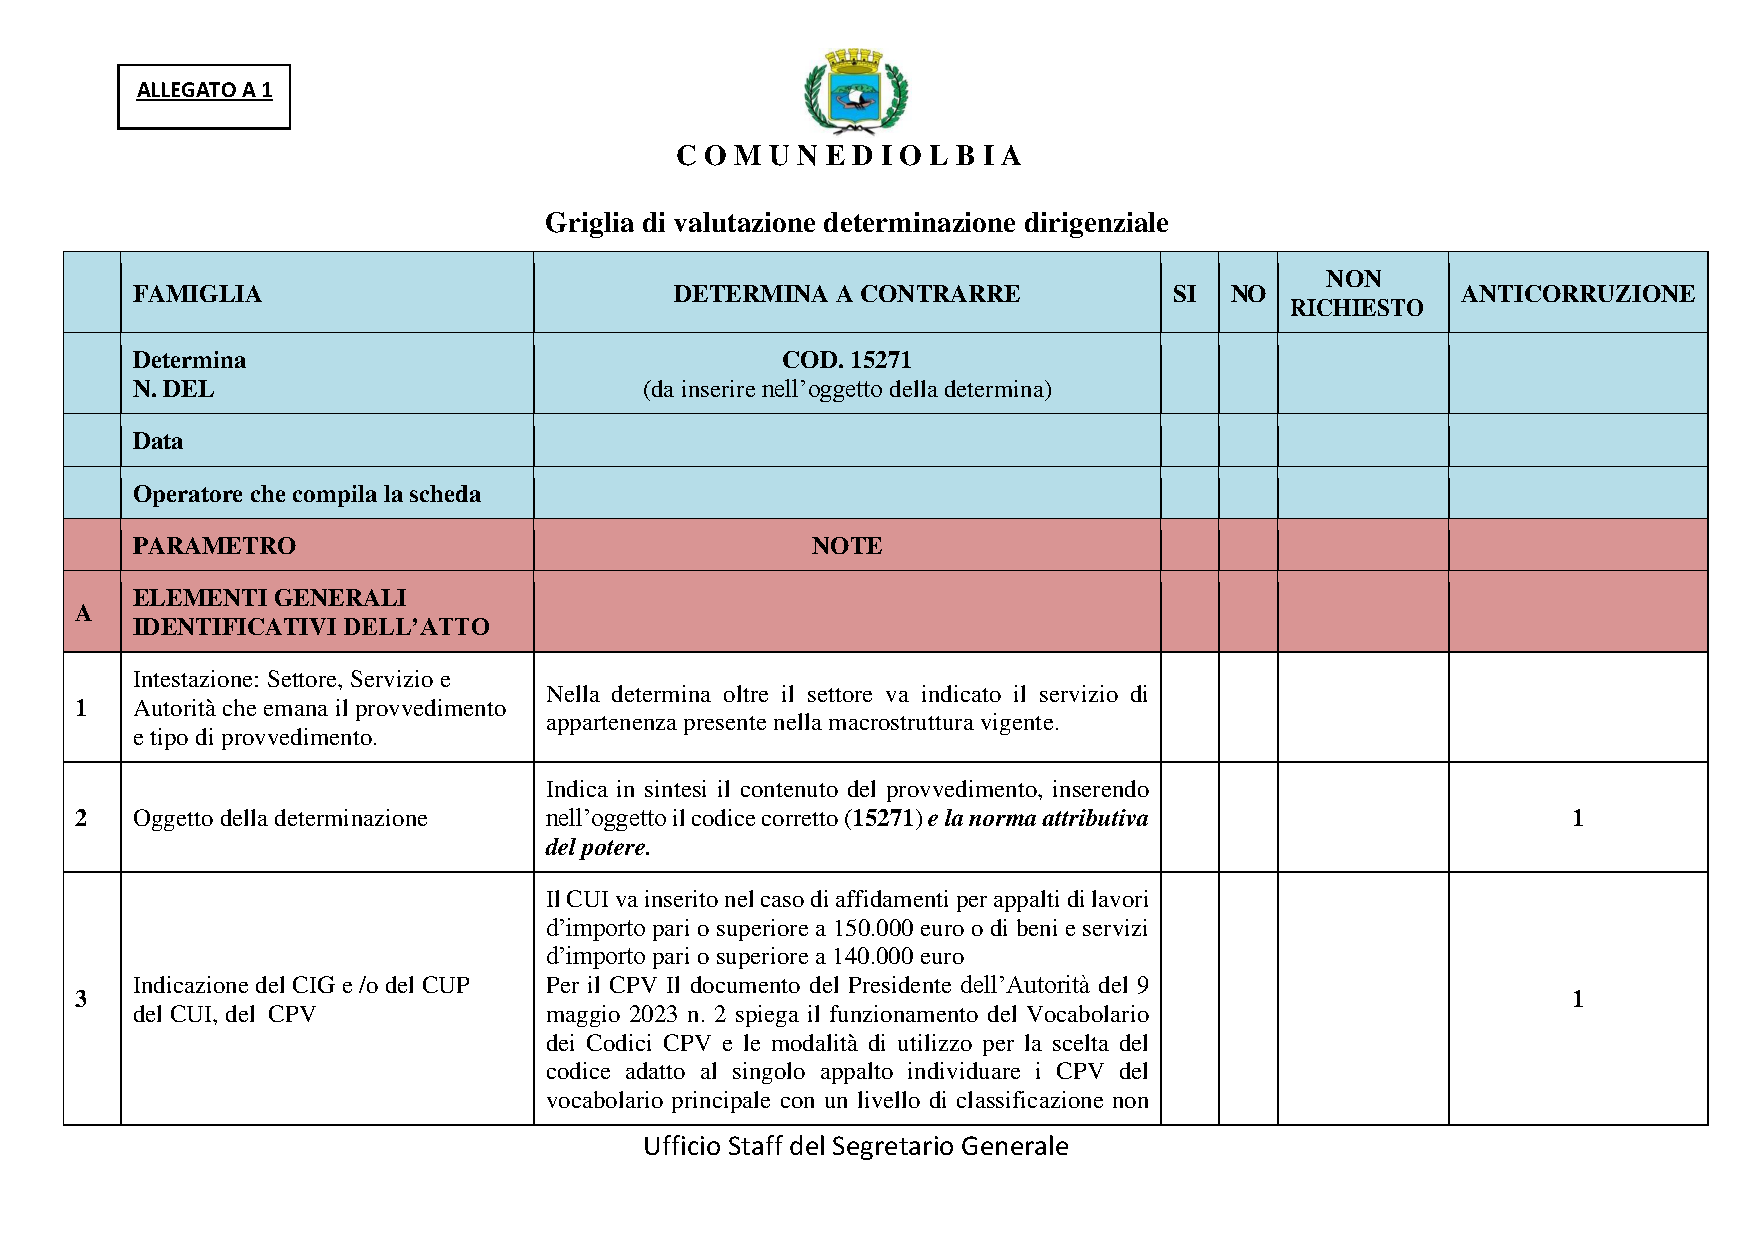
\includepdf[pages=-,scale=0.8, landscape=true,pagecommand={\section*{}}]{\subfix{../Checklists/Olbia/DeterminaAContrarre}}

%\section*{Affidamenti Diretti}

%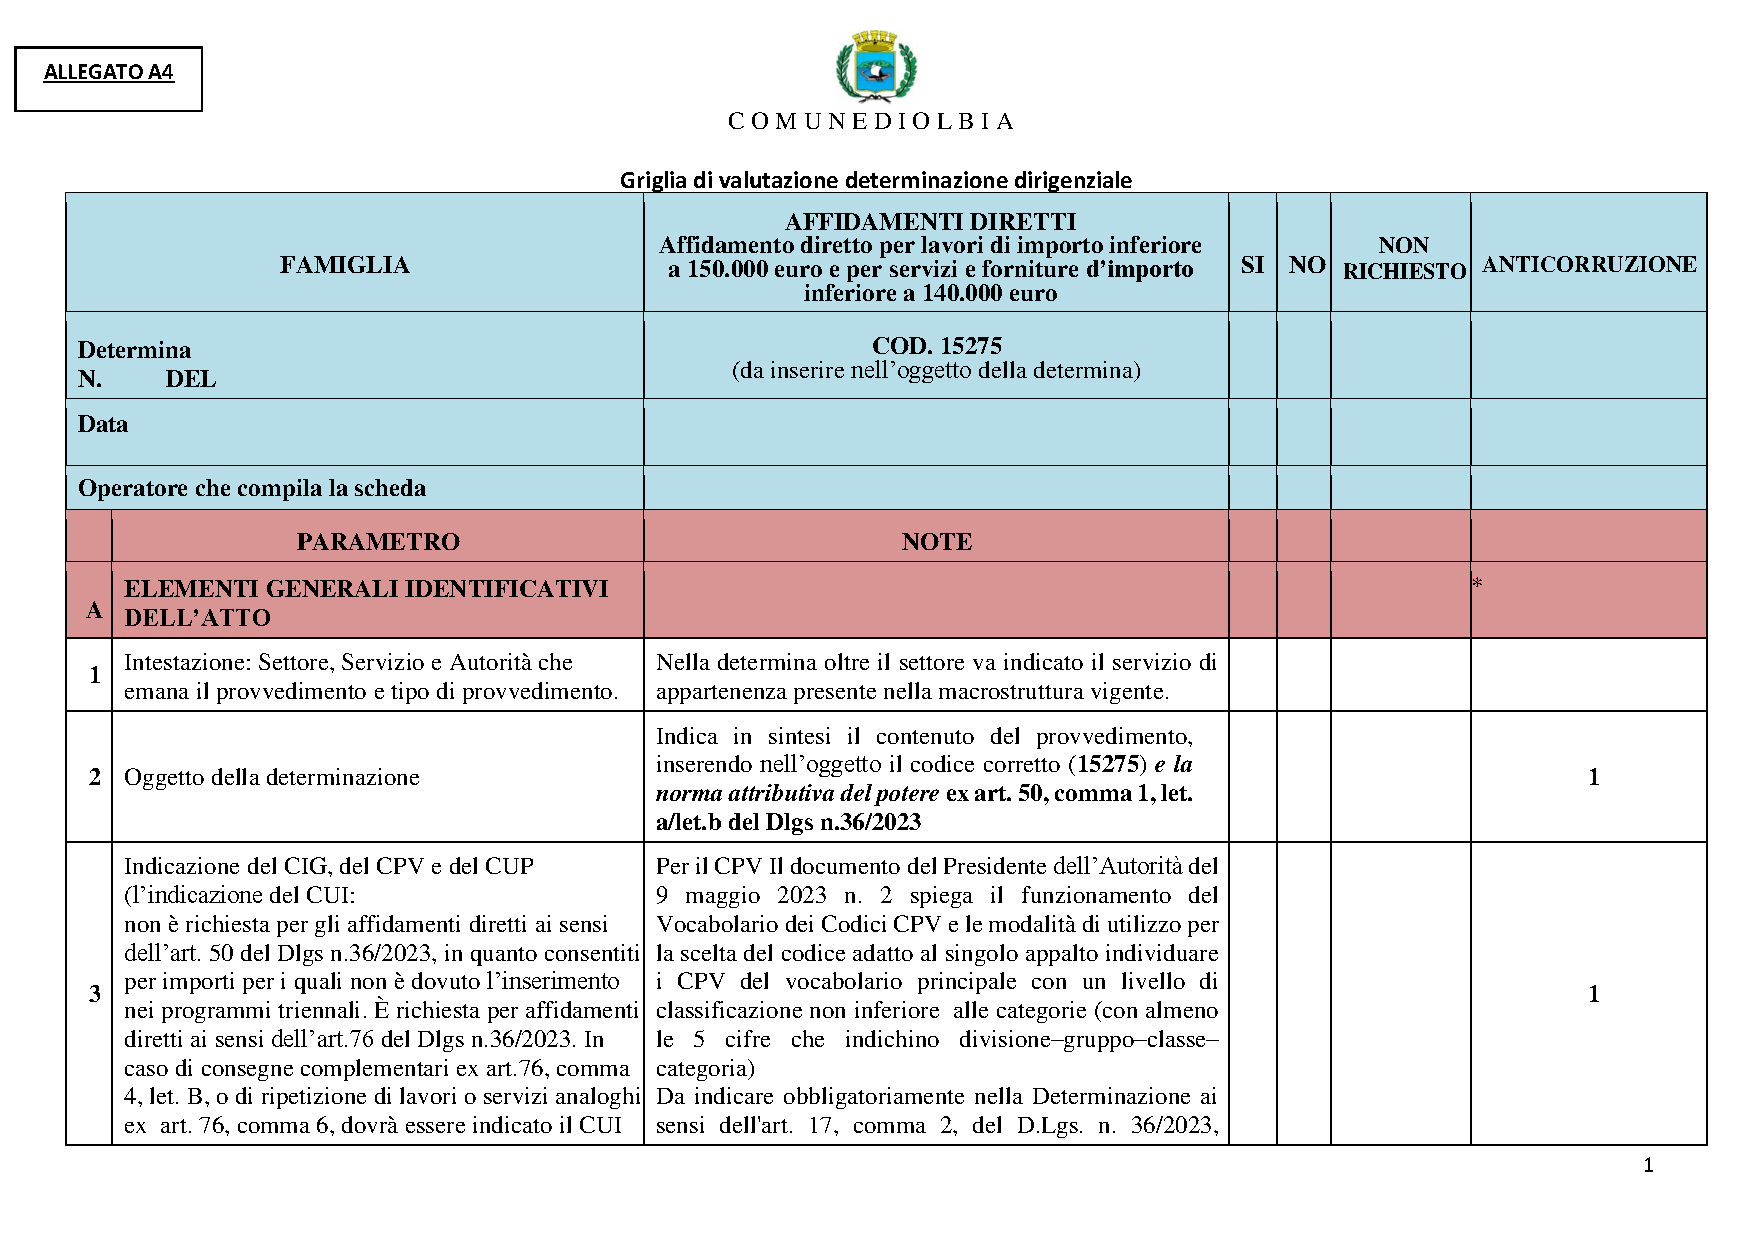
\includepdf[pages=-,scale=0.8, landscape=true,pagecommand={\section*{}}]{\subfix{../Checklists/Olbia/0.AffidamentiDiretti}}

%\section*{Procedura Negoziata}
%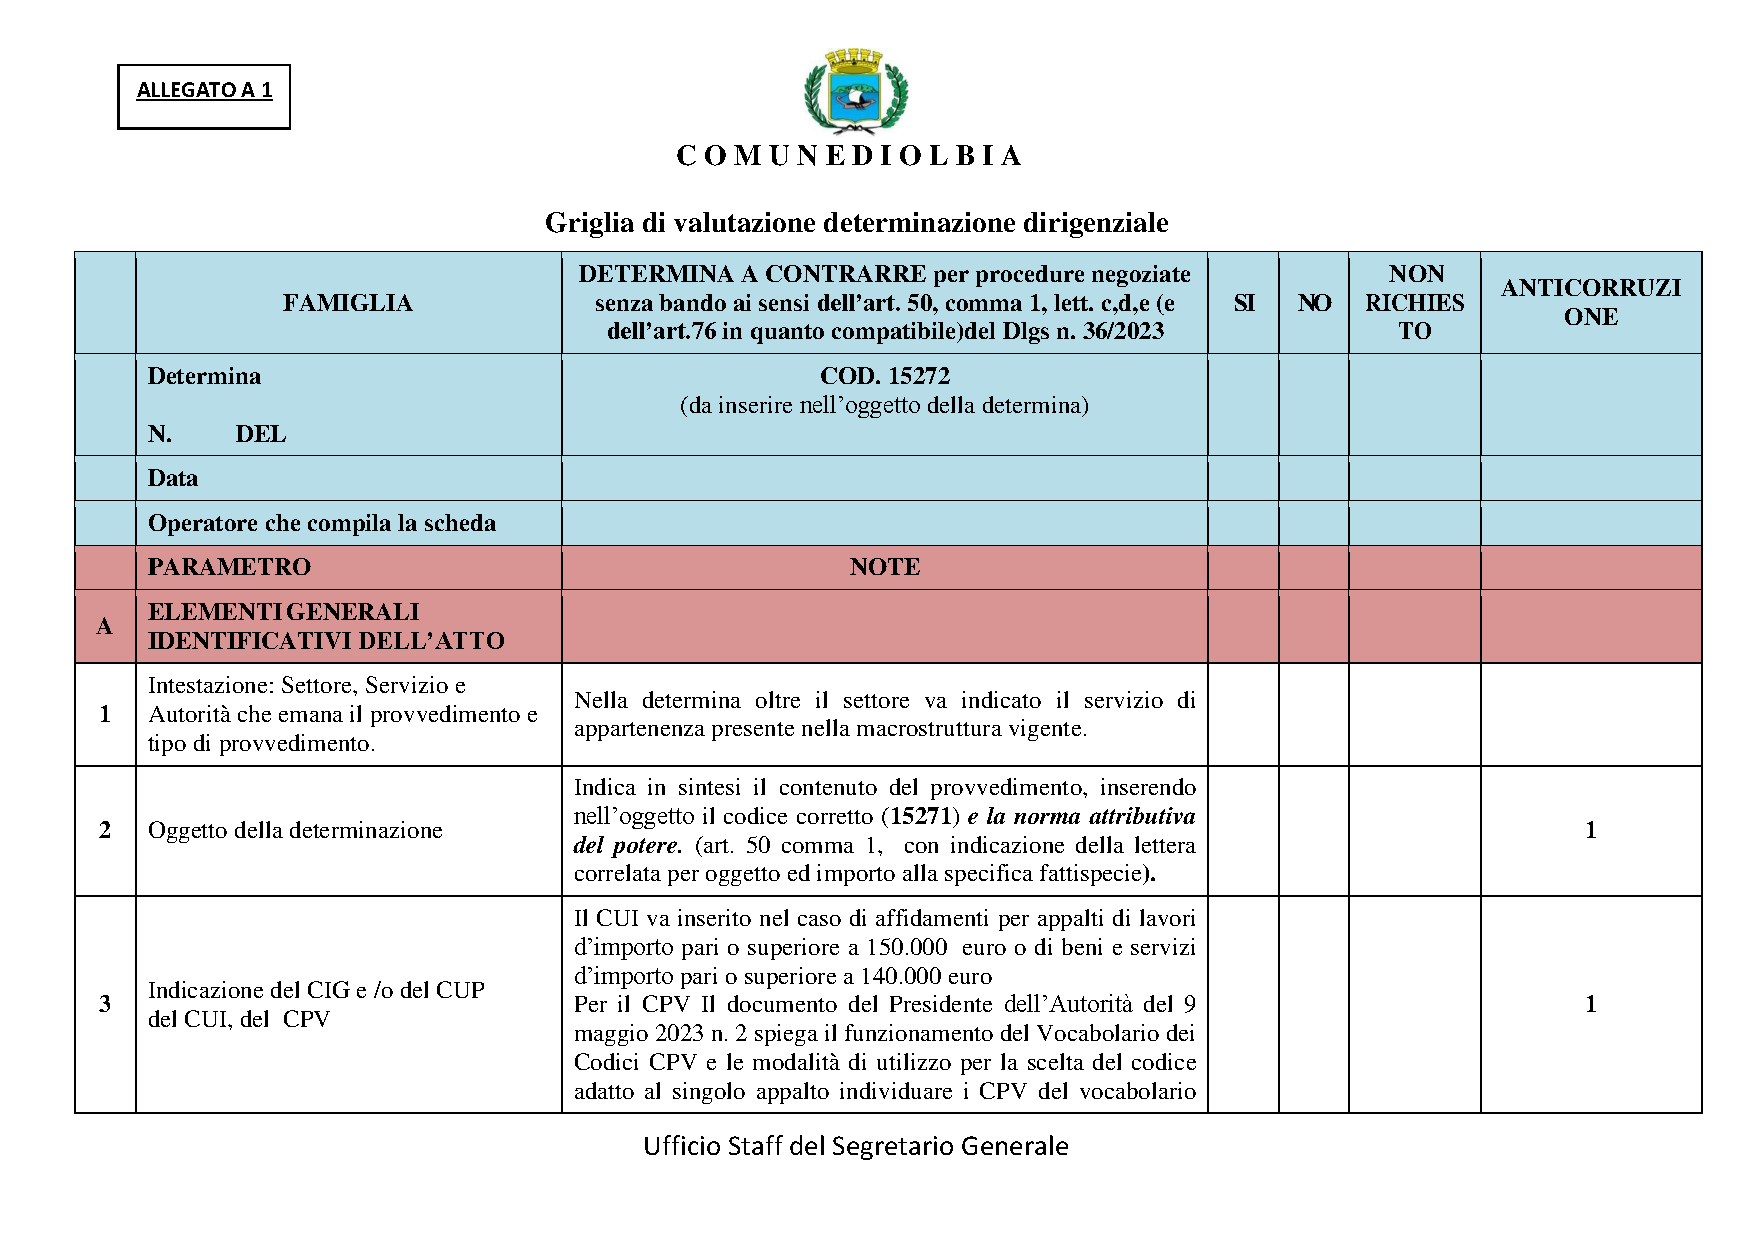
\includepdf[pages=-,scale=0.8, landscape=true,pagecommand={\section*{}}]{\subfix{../Checklists/Olbia/0.ProceduraNegoziata}}

 \end{document}